\setchapterstyle{kao}
\setchapterpreamble[u]{\margintoc}

\chapter{User Interface}
\label{ch:user-interface}

After the main features of the MIDI-Interrupter have been implemented, it needs a way to interact with the user. For debugging purposes, this can be done via the \gls{uart} protocol, but this is not very user-friendly. While there are a lot of possibilities, like a smartphone app which connect via Bluetooth, a Touchscreens display or an high resolution OLED display, the focus was mainly on simplicity. Therefore an \glsunset{lcd}\gls{lcd} in combination with a rotary encoder has been chosen.

\section{The Display}

A \glsreset{lcd}\gls{lcd} makes it very easy to show text or other ASCII symbols due to its builtin HD44780U controller. This controller provides a layer of abstraction to the individual pixels, which makes it possible to send high-level commands to write to the display. Such commands include \cinl{clear display}, \cinl{return home}, or \cinl{function set}.

To connect the display to the \gls{mcu}, three control pins and either four or eight data pins are required. The pins \cinl{D0} to \cinl{D7} are the data pins. To save four pins, the controller offers a 4-bit mode in which only \cinl{D4} to \cinl{D7} are used by serializing the communication and sending the low \gls{nibble} after the high \gls{nibble}. The \cinl{RS} pin selects if the register to operate on is the data or instruction register, the \cinl{RW} pin chooses if this register is read from or written to, and lastly, the \cinl{E} pin starts any read or write operation.

Additionally, the \cinl{VSS} and \cinl{VDD} pins supplies the controller chip with 5V and the \cinl{V0} pin sets the contrast depending on the applied voltage. Finally, the \cinl{A} and \cinl{K} pin are the anode and cathode of the backlight LED and can be directly connected to +5V and ground, since the module already has a builtin series resistor.

\begin{marginfigure}[-7cm]
    \centering
    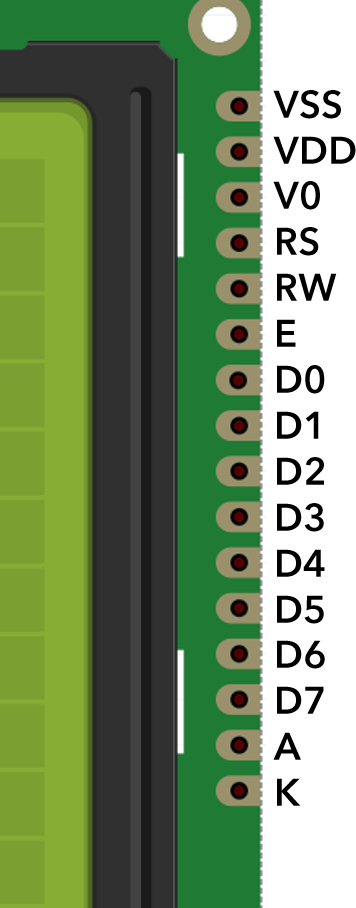
\includegraphics[width=0.5\textwidth]{felix/resources/lcd_pins.png}
    \caption{Pins of an LCD}
    \label{fig:lcd_pins}
\end{marginfigure}

\subsection{Communication}

After power on and automatic initialization of the controller, it has to be set to 4-bit mode with the \cinl{function set} command. After setting other options, like the size of the display or the cursor shape, text can be printed to the display by writing data to the data register. A complete list of all commands and more details on the initialization process can be found in the datasheet, whose URL can be found in QR code \newqrcode{https://www.sparkfun.com/datasheets/LCD/HD44780.pdf}{HD44780 LCD driver datasheet}. % maybe put in sidenote?

Instead of implementing this communication layer from scratch, a very popular library written by Peter Fleury has been used\sidenote{A URL to the library documentation can be found in QR code \newqrcode{http://www.peterfleury.epizy.com/doxygen/avr-gcc-libraries/group__pfleury__lcd.html}{LCD library}}. In \cinl{lcd.h} the used mode and the port and pin number of each pin has to be specified. After that, it is very easy to use the \gls{lcd} as shown in listing \ref{lst:lcdlibrary}

\begin{lstlisting}[caption=LCD Library, label=lst:lcdlibrary]
#include "lcd.h"

int main() {
    lcd_init(LCD_DISP_ON_CURSOR);   // Initializes LCD
    lcd_clrscr();       // Clears the screen
    lcd_home();         // Moves the cursor to position (0,0)
    lcd_puts("Hello there"); // Prints text to the screen
    return 0;
}
\end{lstlisting}

\section{The Rotary Encoder}

After the list of files can be shown on the \gls{lcd}, the user has to be able to cycle through the list and select a file. A relative rotary encoder is the perfect tool for this, because it can rotate endlessly, has clearly noticable discrete steps, a digital output signal and an integrated button to confirm the selection.

In total, the rotary encoder has five pins - two for the supply voltage, one for the button and two for the rotary encoding, \cinl{CLK} and \cinl{DT}. While the naming clearly implies that the \cinl{CLK} signal should be thought of as the main signal, in practice they are completely interchangeable. Figure \ref{fig:rotary-encoder} shows the internal working of the device as well as the resulting \cinl{CLK} and \cinl{DT} signals when the encoder is turned.

\begin{figure}[h!]
    \centering
    \resizebox{\textwidth}{!}{
    \begin{tikztimingtable}[timing/xunit=.5cm, timing/slope=.05, timing/yunit=5mm, line width=1.25pt]
      \raisebox{1.5mm}{CLK} & 4h4l6h 2S 6h4l4h\\
      \raisebox{1.5mm}{DT} &  6h4l4h 2S 4h4l6h\\
        \extracode
      \tikzset{shift={(-4cm,-3mm)}}
      \fill[black!25] (0,0) circle (2cm);
      \fill[white] (0,0) circle (.8cm);
      \foreach \a in {0,36,72,...,360}{
        \draw[black, fill=white, ultra thick] (\a+10:1cm) -- (\a+10:1.8cm) arc(\a+10:\a-10:1.8cm) -- (\a-10:1cm) arc(\a-10:\a+10:1cm);
        \fill[white] (\a+8:2.1cm) -- (\a+18:1.9cm) -- (\a+28:2.1cm);
      }
      \fill[black!50, rounded corners=1pt] (80:2.12cm) -- (90:1.92cm) -- (100:2.12cm) -- ++(0,.2cm) -- ++(.73cm,0) -- (80:2.1cm);
      \draw[semithick] (90:2.3cm) -- ++(.3cm,.05cm) -- ++(-.6cm,.1cm) -- ++(.6cm,.1cm) -- ++(-.6cm,.1cm) -- ++(.3cm,.05cm) node(spring){};
      \draw[thick] (spring) ++(-.4cm,.1mm) -- ++(.9cm,0);
      \foreach \x in {0,.2,...,.8}{
        \draw[semithick] (spring) ++(-\x cm + .4cm,0) -- ++(1mm,1mm);
      }
       \draw[{Stealth[length=10mm, width=1mm]}-, semithick] (5:1.4cm) -- ++(1.3cm,4mm);
       \draw[{Stealth[length=10mm, width=1mm]}-, semithick] (-5:1.4cm) -- ++(1.5cm,-3mm);
      \draw[->,very thick] (5.1cm,1.35cm) arc (240:-60:4mm);
      \draw[<-,very thick] (10.1cm,1.35cm) arc (240:-60:4mm);
      \fill (54:1.5cm) circle (.75mm);
      \draw[semithick] (54:1.5cm) -- ++(.75cm,.75cm) -- ++(7mm,0) node[xshift=-3.5mm,yshift=2mm]{GND};
    \end{tikztimingtable}}
    \caption{Internal working of a rotary encoder}
    \label{fig:rotary-encoder}
\end{figure}

The easiest way to read the signal from the decoder is to set an interrupt on the falling edge\sidenote{Setting it on the rising edge would work equally well, however then the following logic would have to be inverted.} of the \cinl{CLK} signal and read the \cinl{DT} signal at this point. If it's high, the encoder has been turned clockwise, and if it's low it has been turned counter-clockwise.

To confirm the selection, the integrated button, which can be activated by pressing down on the rotary shaft has been used. It was connected to the external interrupt pin \cinl{PD3} on the ATmega2560, which was configured to trigger on a rising edge. The de-bouncing was implemented by adding a 50\,ms delay in the \gls{isr} and clear any pending interrupt on this pin by setting the corresponding bit in the \cinl{EIFR} register.